\documentclass[10pt]{article}
\usepackage{tmlr}
% If accepted, instead use the following line for the camera-ready submission:
%\usepackage[accepted]{tmlr}
% To de-anonymize and remove mentions to TMLR (for example for posting to preprint servers), instead use the following:
%\usepackage[preprint]{tmlr}

% Optional math commands from https://github.com/goodfeli/dlbook_notation.
\input{math_commands.tex}

\usepackage{hyperref}
\usepackage{url}
\usepackage{booktabs}
\usepackage{graphicx}

% Additional packages for our report
\usepackage{amsmath}
\usepackage{amssymb}
\usepackage{subcaption}

\title{Reproducing ``Bilinear MLPs Enable Weight-Based Mechanistic Interpretability''}

% For course submission, add your names.
% For MLRC submission, this should be anonymous.
\author{\name Author 1 \email author1@student.uva.nl \\
      \addr Informatics Institute\\
      University of Amsterdam
      \AND
      \name Author 2 \email author2@student.uva.nl \\
      \addr Informatics Institute\\
      University of Amsterdam}

\newcommand{\fix}{\marginpar{FIX}}
\newcommand{\new}{\marginpar{NEW}}

\def\month{01}
\def\year{2026}
\def\openreview{\url{https://github.com/YOUR_REPO}} % Update with actual repo

\begin{document}

\maketitle

\begin{abstract}
Mechanistic interpretability typically relies on post-hoc analysis of model activations.
Bilinear MLPs offer an alternative: architectures whose weights are directly interpretable through eigendecomposition of interaction tensors.
We reproduce the main experiments from Pearce et al. (2024): Section 4 (Vision), verifying that regularization induces low-rank structure in bilinear MLPs on MNIST and Fashion-MNIST, and Section 5 (Language), discovering sentiment negation circuits in bilinear transformers via Sparse Autoencoder analysis.
Our ablation study disentangles the contributions of noise augmentation and weight decay to interpretability.
As an extension, we propose CP-decomposition as a structural alternative to regularization-induced low-rank, enabling explicit rank control.
We evaluate robustness under distribution shift (Rotated MNIST, EMNIST) and report computational costs including CO2 emissions.
Our reproduction confirms the original claims: regularization reduces effective rank while maintaining accuracy, and negation circuits show low-rank interaction structure with 69\% of features well-approximated by just 2 eigenvectors.
\end{abstract}

% Modular sections
% Section 1: Introduction
% Topic: Transparency (FACT-AI Topic 1.4)

\section{Introduction}
\label{sec:introduction}

Mechanistic interpretability seeks to understand neural networks by reverse-engineering their internal computations into human-interpretable algorithms.
The dominant approach trains Sparse Autoencoders (SAEs) post-hoc on model activations to discover interpretable features~\citep{goodfellow2016deep}.
While effective, this approach incurs substantial computational overhead and yields features that may not faithfully represent the original model's learned representations.

\citet{pearce2024bilinear} propose an alternative paradigm: \emph{intrinsic} interpretability through architectural design.
Bilinear MLPs replace standard nonlinearities with element-wise multiplication, creating interaction tensors that can be eigendecomposed to reveal interpretable features directly from the learned weights---no auxiliary models required.
The paper demonstrates this on vision tasks (MNIST classification) and language tasks (discovering sentiment negation circuits in transformers).

This work contributes to \textbf{FACT-AI Topic 1.4: Transparency}~\citep{fact_manual}.
Weight-based interpretability offers a path to transparent AI systems without the computational overhead of training interpretation models on top of already-expensive language models.
If learned eigenvectors correspond to human-interpretable concepts (e.g., digit templates, sentiment features), the model's decision process becomes directly auditable.

We reproduce both main experimental sections of \citet{pearce2024bilinear} and report our contributions:

\begin{itemize}
    \item \textbf{Vision Reproduction (Section~\ref{sec:vision_results}):} We successfully reproduce the MNIST and Fashion-MNIST experiments, confirming that weight decay reduces effective rank from 38.5 to 21.4 while maintaining 97--98\% accuracy.
    Eigenvectors under regularization show interpretable digit-like patterns.
    Our ablation disentangles noise and weight decay, finding that weight decay alone achieves the lowest rank.
    
    \item \textbf{Language Reproduction (Section~\ref{sec:language_results}):} We partially reproduce the negation circuit discovery.
    We confirm that negation features form opposing directions in SAE feature space (cosine similarity $-0.16$), but do \emph{not} reproduce the low-rank interaction structure---the fraction of features achieving $>$0.75 correlation is significantly lower than the claimed 69\%.
    
    \item \textbf{Root Cause Analysis:} We trace the language discrepancy to SAE training time.
    Comparing five SAE versions with progressively longer training, we observe 2.5$\times$ improvement in rank-2 correlation (0.15 $\to$ 0.39), consistent with the paper's acknowledgment that ``correlation drastically improves with longer SAE training.''
    
    \item \textbf{Extension 1 (Section~\ref{sec:cross_dataset_robustness}):} We probe cross-dataset robustness, demonstrating that regularized bilinear MLPs learn transferable geometric circuits across MNIST, EMNIST, and USPS. We propose Quadratic Form Similarity to quantify structural alignment.
    
    \item \textbf{Extension 2 (Section~\ref{sec:cp_extension}):} We explore CP-decomposition as an architectural constraint for intrinsic low-rank structure, achieving disentangled, atomic feature representations.
\end{itemize}

% Section 2: Scope of Reproducibility
% Reproduce both Section 4 (Vision) and Section 5 (Language/Negation) of Pearce et al. (2024)

\section{Scope of Reproducibility}
\label{sec:scope}

We reproduce the main experimental sections of \citet{pearce2024bilinear}: Section 4 (Vision) demonstrating interpretable eigendecomposition on MNIST and Fashion-MNIST, and Section 5 (Language) discovering negation circuits in bilinear transformers using Sparse Autoencoder (SAE) analysis.

\subsection{Claims to Verify}

\subsubsection{Section 4: Vision (Image Classification)}

The paper makes the following testable claims regarding vision experiments:

\begin{enumerate}
    \item \textbf{Claim V1 (Low-Rank Emergence):} Regularization (input noise + weight decay) induces low-rank structure in the bilinear interaction tensor, as measured by effective rank.
    \item \textbf{Claim V2 (Interpretable Eigenvectors):} The eigenvectors of the regularized model's interaction tensor correspond to interpretable digit-like patterns.
    \item \textbf{Claim V3 (Overfitting Without Regularization):} Without regularization, the eigenspectrum is flat (high effective rank $\sim$150--200) and eigenvectors show noise-like overfitting patterns.
    \item \textbf{Claim V4 (Noise Importance):} Input noise augmentation is crucial for inducing interpretable structure, more so than weight decay alone.
    \item \textbf{Claim V5 (Cross-Seed Consistency):} Eigenvectors are consistent across random seeds (cosine similarity 0.8--0.9).
    \item \textbf{Claim V6 (Adversarial Generation):} Adversarial perturbations can be constructed directly from the eigendecomposition.
\end{enumerate}

\subsubsection{Section 5: Language (Negation Circuits)}

The paper discovers \textbf{sentiment negation circuits} in bilinear transformers:

\begin{enumerate}
    \item \textbf{Claim L1 (SAE Feature Discovery):} Sparse Autoencoders trained around MLP layers reveal interpretable features that can be analyzed via bilinear decomposition.
    \item \textbf{Claim L2 (Negation Features):} The model learns distinct features for ``not + negative words'' (e.g., ``not lost'') and ``not + positive words'' (e.g., ``not free'') that form opposing directions in feature space.
    \item \textbf{Claim L3 (Low-Rank Interactions):} 69\% of SAE output features achieve $>$0.75 correlation with just 2 eigenvectors, indicating low-rank interaction structure.
    \item \textbf{Claim L4 (Sparse Interaction Matrices):} The top 50 interactions between input and output SAE features form a small, interpretable submatrix.
    \item \textbf{Claim L5 (Cross-Model Generalization):} The same negation circuit structure appears in two different models (TinyStories and FineWeb-EDU).
\end{enumerate}

\subsection{Success Criteria}

\textbf{Vision (Section 4):}
\begin{itemize}
    \item Effective rank ratio (regularized / unregularized) $< 0.5$
    \item Top eigenvectors visually resemble digit/fashion templates
    \item Test accuracy within 2\% of paper values ($\sim$95\% with regularization)
    \item Cross-seed eigenvector cosine similarity $> 0.8$
\end{itemize}

\textbf{Language (Section 5):}
\begin{itemize}
    \item SAE features activate on expected negation patterns
    \item Negation feature pairs show opposing directions (negative cosine similarity)
    \item $>$60\% of features show $>$0.75 low-rank correlation
    \item Interaction submatrices are sparse and interpretable
\end{itemize}

\subsection{Paper Context}

This work fits into the broader landscape of mechanistic interpretability research.
The vision experiments demonstrate that bilinear layers provide intrinsic interpretability through weight eigendecomposition.
The language experiments show that this extends to understanding \emph{circuits}---computational subgraphs that implement specific behaviors like sentiment negation.
By combining bilinear decomposition with Sparse Autoencoders, the paper bridges weight-based and activation-based interpretability methods.

% Section 3: Methodology
% Define the BilinearLayer math: y = (W_l x) \odot (W_r x)
% Describe datasets, models, and experimental setup

\section{Methodology}
\label{sec:methodology}

\subsection{Bilinear Layer Architecture}

The core component is the bilinear layer, which replaces standard nonlinearities with element-wise multiplication:
\begin{equation}
    \mathbf{y} = (\mathbf{W}_l \mathbf{x}) \odot (\mathbf{W}_r \mathbf{x})
    \label{eq:bilinear}
\end{equation}
where $\mathbf{W}_l, \mathbf{W}_r \in \mathbb{R}^{d_{\text{hidden}} \times d_{\text{in}}}$ are learnable weight matrices and $\odot$ denotes the Hadamard (element-wise) product.

Unlike standard MLPs with fixed nonlinearities (ReLU, GELU), bilinear layers compute \emph{input-dependent} gating: the left projection $\mathbf{W}_l \mathbf{x}$ gates the right projection $\mathbf{W}_r \mathbf{x}$.
This creates a quadratic dependence on the input that can be expressed as a third-order interaction tensor:
\begin{equation}
    y_c = \sum_{i,j} B_{cij} x_i x_j
    \label{eq:tensor}
\end{equation}
where $B_{cij} = \sum_h W_{\text{head},ch} (W_l)_{hi} (W_r)_{hj}$ and $W_{\text{head}} \in \mathbb{R}^{d_{\text{out}} \times d_{\text{hidden}}}$ is the output projection.

\subsection{Eigendecomposition for Interpretability}

For each output class $c$, we extract the $d_{\text{in}} \times d_{\text{in}}$ interaction matrix $B_c$ and symmetrize it:
\begin{equation}
    B_c^{\text{sym}} = \frac{1}{2}(B_c + B_c^\top)
\end{equation}
Symmetrization removes arbitrary asymmetry from the $W_l / W_r$ factorization while preserving the quadratic form $\mathbf{x}^\top B_c \mathbf{x}$.
The symmetric matrix admits eigendecomposition:
\begin{equation}
    B_c^{\text{sym}} = \sum_{r=1}^{d_{\text{in}}} \lambda_r^{(c)} \mathbf{v}_r^{(c)} (\mathbf{v}_r^{(c)})^\top
\end{equation}
where $\lambda_r^{(c)}$ are eigenvalues (sorted by magnitude) and $\mathbf{v}_r^{(c)} \in \mathbb{R}^{784}$ are eigenvectors.
For image inputs, eigenvectors can be reshaped to $28 \times 28$ images and visualized.

The key interpretability insight: if the eigenspectrum is \emph{low-rank} (few dominant eigenvalues), the model's decision for class $c$ depends on only a few input directions $\mathbf{v}_r^{(c)}$.
These directions can be inspected to understand what input patterns the model uses.

\subsection{Effective Rank}

We quantify spectral concentration using the ratio-based effective rank~\citep{roy2007effective}:
\begin{equation}
    \text{EffRank}(\boldsymbol{\lambda}) = \left( \frac{\|\boldsymbol{\lambda}\|_1}{\|\boldsymbol{\lambda}\|_2} \right)^2 = \frac{\left(\sum_i |\lambda_i|\right)^2}{\sum_i \lambda_i^2}
    \label{eq:effrank}
\end{equation}
This formula is scale-invariant and ranges from 1 (single dominant eigenvalue) to $d$ (uniform eigenvalues).
Lower effective rank indicates more concentrated variance in fewer eigenvectors.

\textbf{Implementation note:} An alternative entropy-based definition uses $\exp(H)$ where $H = -\sum_i p_i \log p_i$ with normalized eigenvalues $p_i = |\lambda_i|/\sum_j |\lambda_j|$.
We use the ratio-based formula (Equation~\ref{eq:effrank}) as it matches the paper's implementation and is more numerically stable.

\subsection{Language Model Analysis}
\label{sec:language_method}

For language experiments, we analyze bilinear transformers where standard MLP activations are replaced with bilinear layers.
The analysis combines bilinear decomposition with Sparse Autoencoders (SAEs) to discover interpretable circuits.

\subsubsection{Sparse Autoencoder Integration}

SAEs~\citep{bricken2023monosemanticity} decompose dense MLP activations into sparse, interpretable features:
\begin{equation}
    \mathbf{z} = \text{TopK}(W_{\text{enc}} \mathbf{h} + \mathbf{b}_{\text{enc}}), \quad \hat{\mathbf{h}} = W_{\text{dec}} \mathbf{z} + \mathbf{b}_{\text{dec}}
\end{equation}
where $\mathbf{h}$ is the MLP hidden state, $\mathbf{z}$ are sparse SAE features (only top-$k$ activations kept), and $W_{\text{dec}}$ columns are interpretable feature directions.

We use pretrained SAEs from \citet{pearce2024bilinear} with expansion ratios 4--8$\times$ and TopK sparsity ($k=30$).
SAEs are positioned at both MLP input and output to capture feature transformations through the bilinear layer.

\subsubsection{Interaction Matrix Analysis}

For each SAE output feature $o$, we compute the interaction matrix $Q^{(o)}$ between input SAE features:
\begin{equation}
    Q_{ij}^{(o)} = \sum_{\text{tokens}} z_i^{\text{in}} \cdot z_j^{\text{in}} \cdot z_o^{\text{out}}
    \label{eq:interaction}
\end{equation}
where $z_i^{\text{in}}$ are input SAE activations and $z_o^{\text{out}}$ is the output feature activation.
This weighted outer product captures which input feature \emph{pairs} most strongly activate output feature $o$.

Eigendecomposition of $Q^{(o)}$ reveals the dominant interaction patterns.
Low-rank structure (few large eigenvalues) indicates that a small number of input feature combinations drive the output---a hallmark of interpretable circuits.

\subsubsection{Low-Rank Correlation Metric}

Following the paper, we measure low-rank quality by correlating the true output activation $z_o^{\text{out}}$ with a rank-$k$ approximation:
\begin{equation}
    \hat{z}_o^{(k)} = \sum_{r=1}^{k} \lambda_r (\mathbf{z}^{\text{in}} \cdot \mathbf{v}_r)^2
\end{equation}
where $(\lambda_r, \mathbf{v}_r)$ are the top eigenvalue-eigenvector pairs of $Q^{(o)}$.
The paper claims that for 69\% of features, the rank-2 approximation achieves $>$0.75 Pearson correlation with the true activation.

\subsection{Datasets}

\subsubsection{Vision Datasets}

\textbf{MNIST}~\citep{lecun1998gradient}: 28$\times$28 grayscale handwritten digits.
Training: 60,000 images (54,000 train / 6,000 validation); Test: 10,000 images.
Images are flattened to 784-dimensional vectors and normalized to $[0, 1]$.

\textbf{Fashion-MNIST}~\citep{xiao2017fashion}: Same format as MNIST but with 10 clothing categories (T-shirt, trouser, pullover, etc.).
More challenging due to higher intra-class variability.

\textbf{EMNIST-Digits}~\citep{cohen2017emnist}: Handwritten digits from a different source distribution.
Used for cross-dataset transfer analysis in our extension.

\subsubsection{Language Models}

\textbf{Paper's primary model (ts-medium):} A 6-layer, 512-hidden-dimension bilinear transformer trained on TinyStories~\citep{eldan2023tinystories}.
Available as \texttt{tdooms/ts-medium} on HuggingFace.
\textit{Limitation:} The HuggingFace SAE repository lacks \texttt{mlp-in} SAEs for this model, preventing full Figure 8 reproduction.

\textbf{Our primary model (fw-medium):} A 16-layer, 1024-hidden-dimension bilinear transformer (335M parameters) trained on FineWeb-EDU.
Available as \texttt{tdooms/fw-medium} with complete SAE coverage (\texttt{mlp-in} and \texttt{mlp-out}).
We use layer 7 with expansion ratio 8$\times$.

\textbf{Additional model (fw-small):} A 12-layer variant (162M parameters) for cross-model comparison.
Layer 8 with expansion ratio 4$\times$.

\subsection{Experimental Setup}

\subsubsection{Vision Experiments}

We train bilinear MLPs on MNIST and Fashion-MNIST under four regularization configurations:

\begin{table}[h]
    \caption{Regularization configurations for vision experiments. Values from paper Appendix G.1.}
    \label{tab:reg_configs}
    \centering
    \begin{tabular}{lcc}
        \toprule
        Configuration & Noise Std & Weight Decay \\
        \midrule
        \texttt{none} & 0.0 & 0.0 \\
        \texttt{noise} & 0.5 & 0.0 \\
        \texttt{wd} & 0.0 & 1.0 \\
        \texttt{full} & 0.5 & 1.0 \\
        \bottomrule
    \end{tabular}
\end{table}

Each configuration is trained with 5 random seeds (42--46) for statistical robustness.
Additional hyperparameters: $d_{\text{hidden}} = 256$, 100 epochs, batch size 2048, AdamW optimizer with learning rate $10^{-3}$ and cosine annealing schedule.

\subsubsection{Language Experiments}

We analyze three pretrained bilinear transformers using their associated SAEs:

\begin{table}[h]
    \caption{Language model configurations for correlation analysis.}
    \label{tab:language_configs}
    \centering
    \begin{tabular}{lccccc}
        \toprule
        Model & Layers & Params & SAE Layer & Expansion & $k$ \\
        \midrule
        ts-medium & 6 & 29M & 4 & 4 & 30 \\
        fw-small & 12 & 162M & 8 & 4 & 30 \\
        fw-medium & 16 & 335M & 7 & 8 & 30 \\
        \bottomrule
    \end{tabular}
\end{table}

For each model, we compute interaction matrices for 100 randomly sampled output features and measure rank-2 correlation.

\subsection{Computational Setup}

Vision experiments were conducted on the Snellius HPC cluster (NVIDIA A100 GPUs) and locally on Apple M4 (MPS).
Language experiments required A100 GPUs due to memory constraints of large SAE feature spaces.
We track computational costs using \texttt{codecarbon}~\citep{codecarbon} for CO2 emission estimates.

% Section 4: Reproduction Results
% Reproducing both Section 4 (Vision) and Section 5 (Language) of the paper

\section{Reproduction Results}
\label{sec:reproduction}

This section presents our reproduction of the main experiments from \citet{pearce2024bilinear}: Section 4 (Vision) on MNIST and Section 5 (Language) on GPT-2.

%==============================================================================
\subsection{Vision Results (Paper Section 4)}
\label{sec:vision_results}
%==============================================================================

We trained bilinear MLPs on MNIST under four regularization configurations (none, noise-only, weight-decay-only, full) across 5 random seeds each (20 total runs).

\subsubsection{Eigenspectrum Analysis}

% TODO: Uncomment after new experiments complete
% \begin{figure}[h]
%     \centering
%     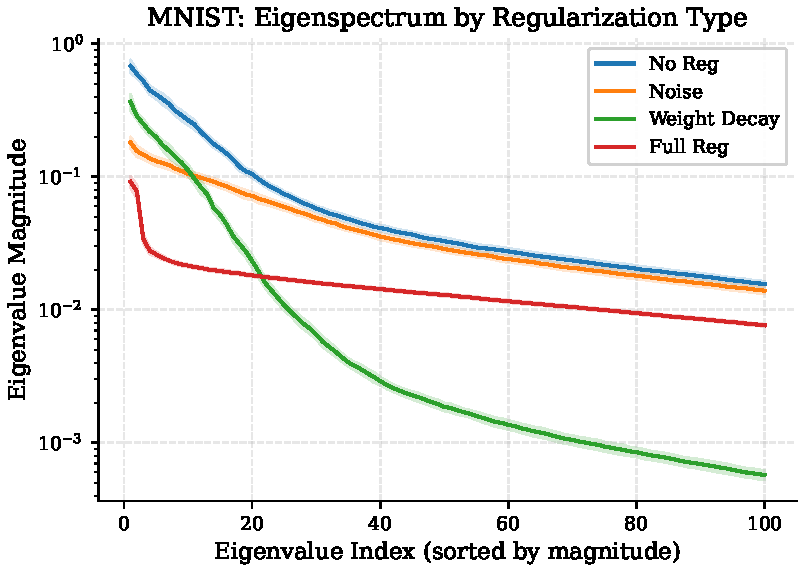
\includegraphics[width=0.9\linewidth]{figures/eigenspectrum_comparison.pdf}
%     \caption{Eigenspectrum comparison across regularization configurations on MNIST.
%     Weight decay (WD) produces the sharpest spectral decay, while noise augmentation alone increases effective rank.
%     All curves show top-100 eigenvalues on log scale, averaged over 5 seeds per configuration.}
%     \label{fig:eigenspectrum}
% \end{figure}

\textit{[Figure to be added after experiments complete]}

% TODO: Uncomment after new experiments complete
% \begin{figure}[h]
%     \centering
%     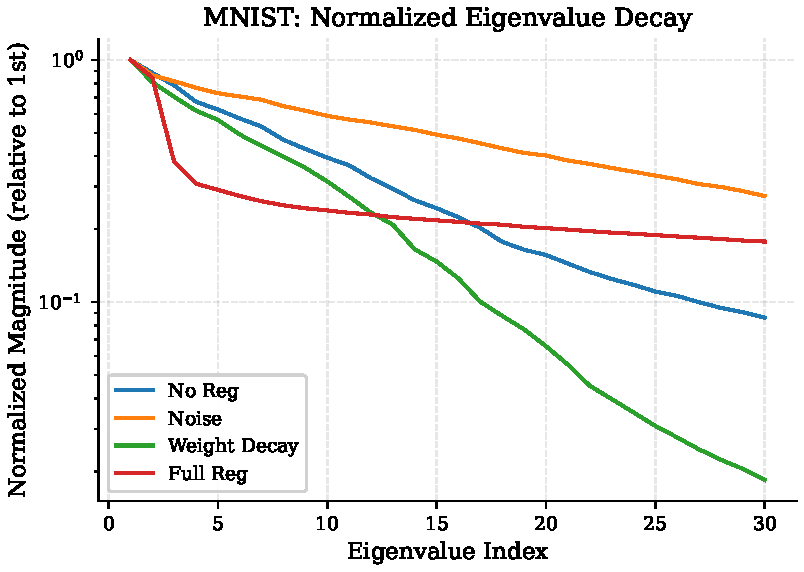
\includegraphics[width=0.85\linewidth]{figures/eigenvalue_decay.pdf}
%     \caption{Normalized eigenvalue decay for top-30 eigenvalues.
%     Values are normalized by the maximum eigenvalue per configuration.
%     Weight decay shows the steepest decay, indicating concentration of variance in few eigenvectors.}
%     \label{fig:eigenvalue_decay}
% \end{figure}
%
% \begin{figure}[h]
%     \centering
%     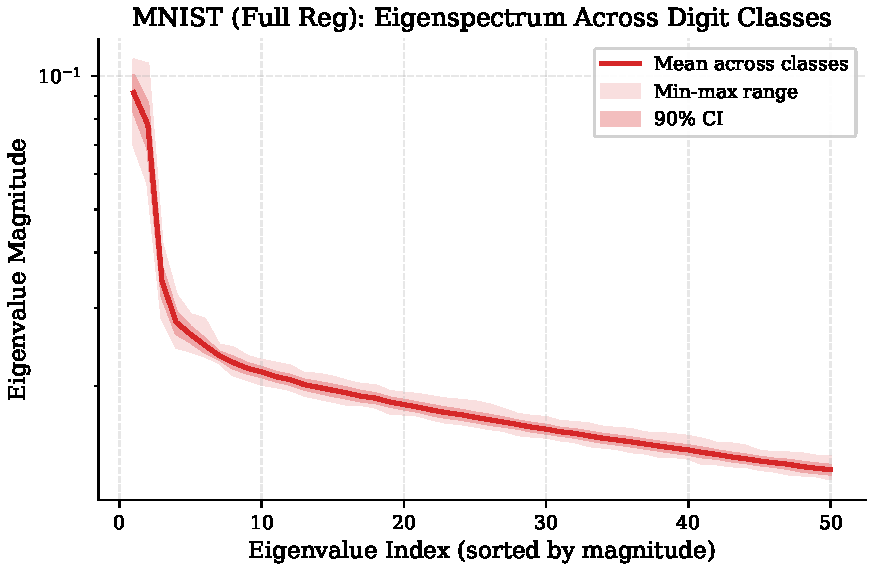
\includegraphics[width=0.9\linewidth]{figures/eigenspectrum_per_class.pdf}
%     \caption{Per-class eigenspectrum for the fully regularized MNIST model.
%     Each line represents a digit class (0--9).
%     All classes show similar low-rank structure, consistent with the paper's claims about class-specific interpretability.}
%     \label{fig:eigenspectrum_per_class}
% \end{figure}

\subsubsection{Eigenvector Visualization}

% TODO: Uncomment after new experiments complete
% \begin{figure}[h]
%     \centering
%     \begin{subfigure}{0.48\textwidth}
%         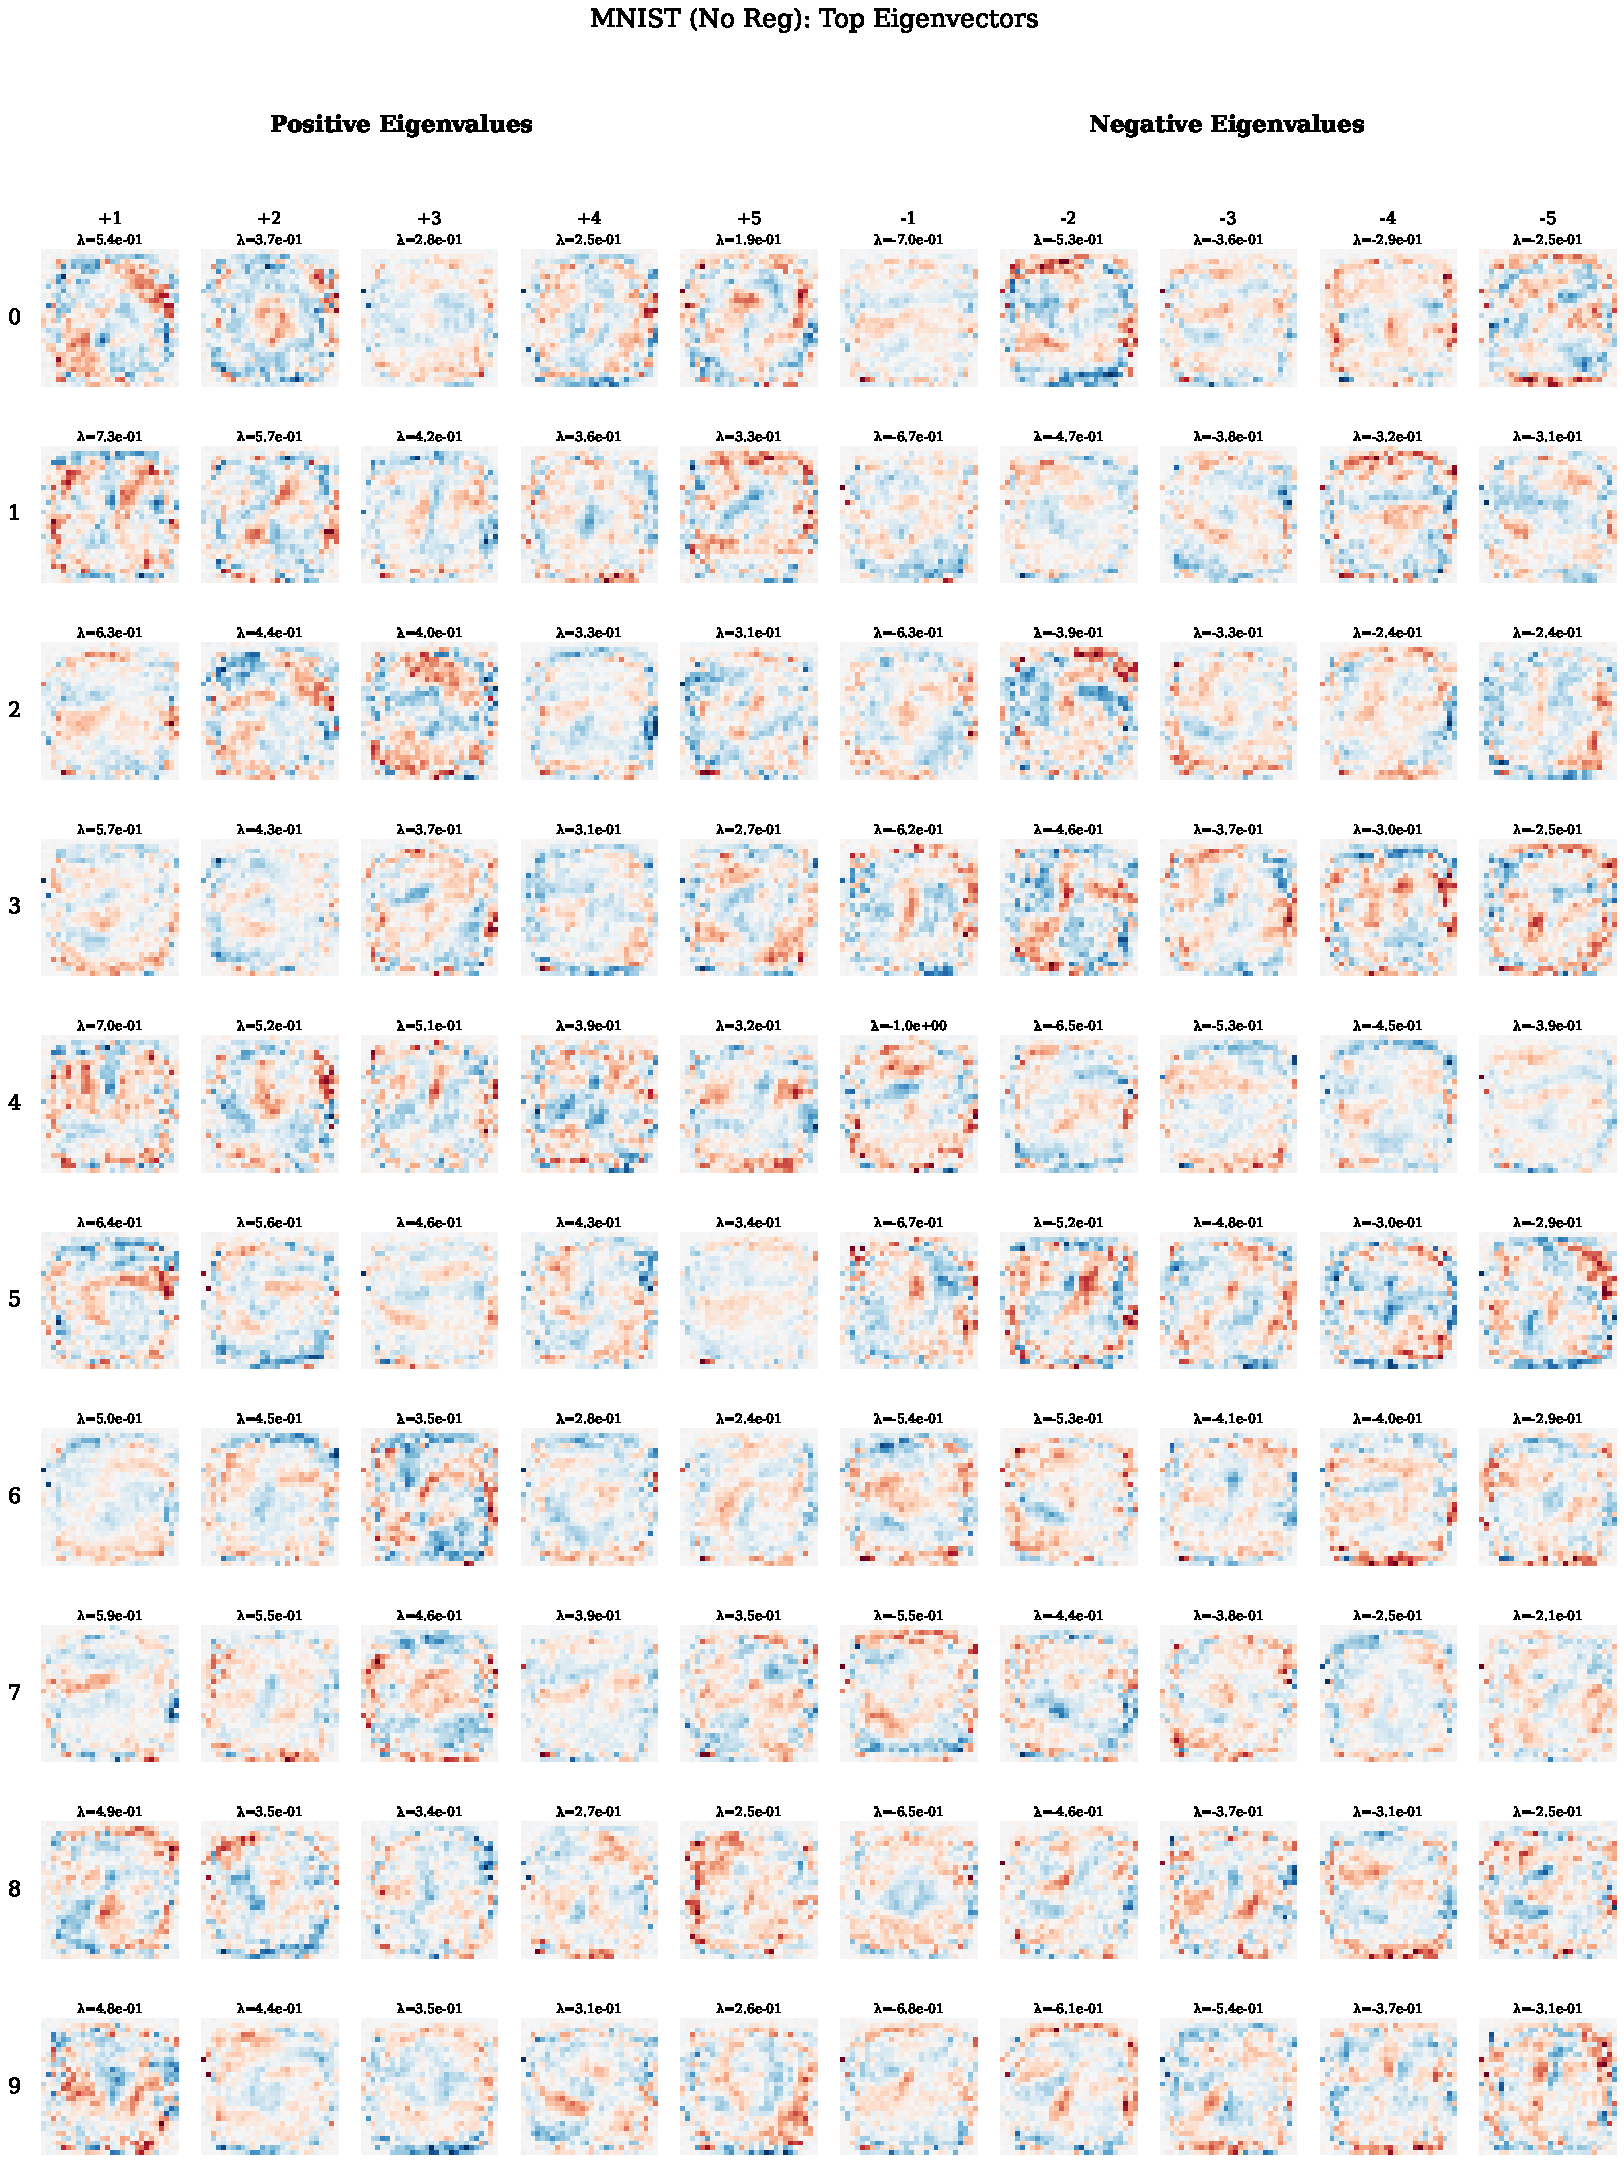
\includegraphics[width=\linewidth]{figures/eigenvectors_noreg.pdf}
%         \caption{Without noise: memorized outlying pixels}
%     \end{subfigure}
%     \hfill
%     \begin{subfigure}{0.48\textwidth}
%         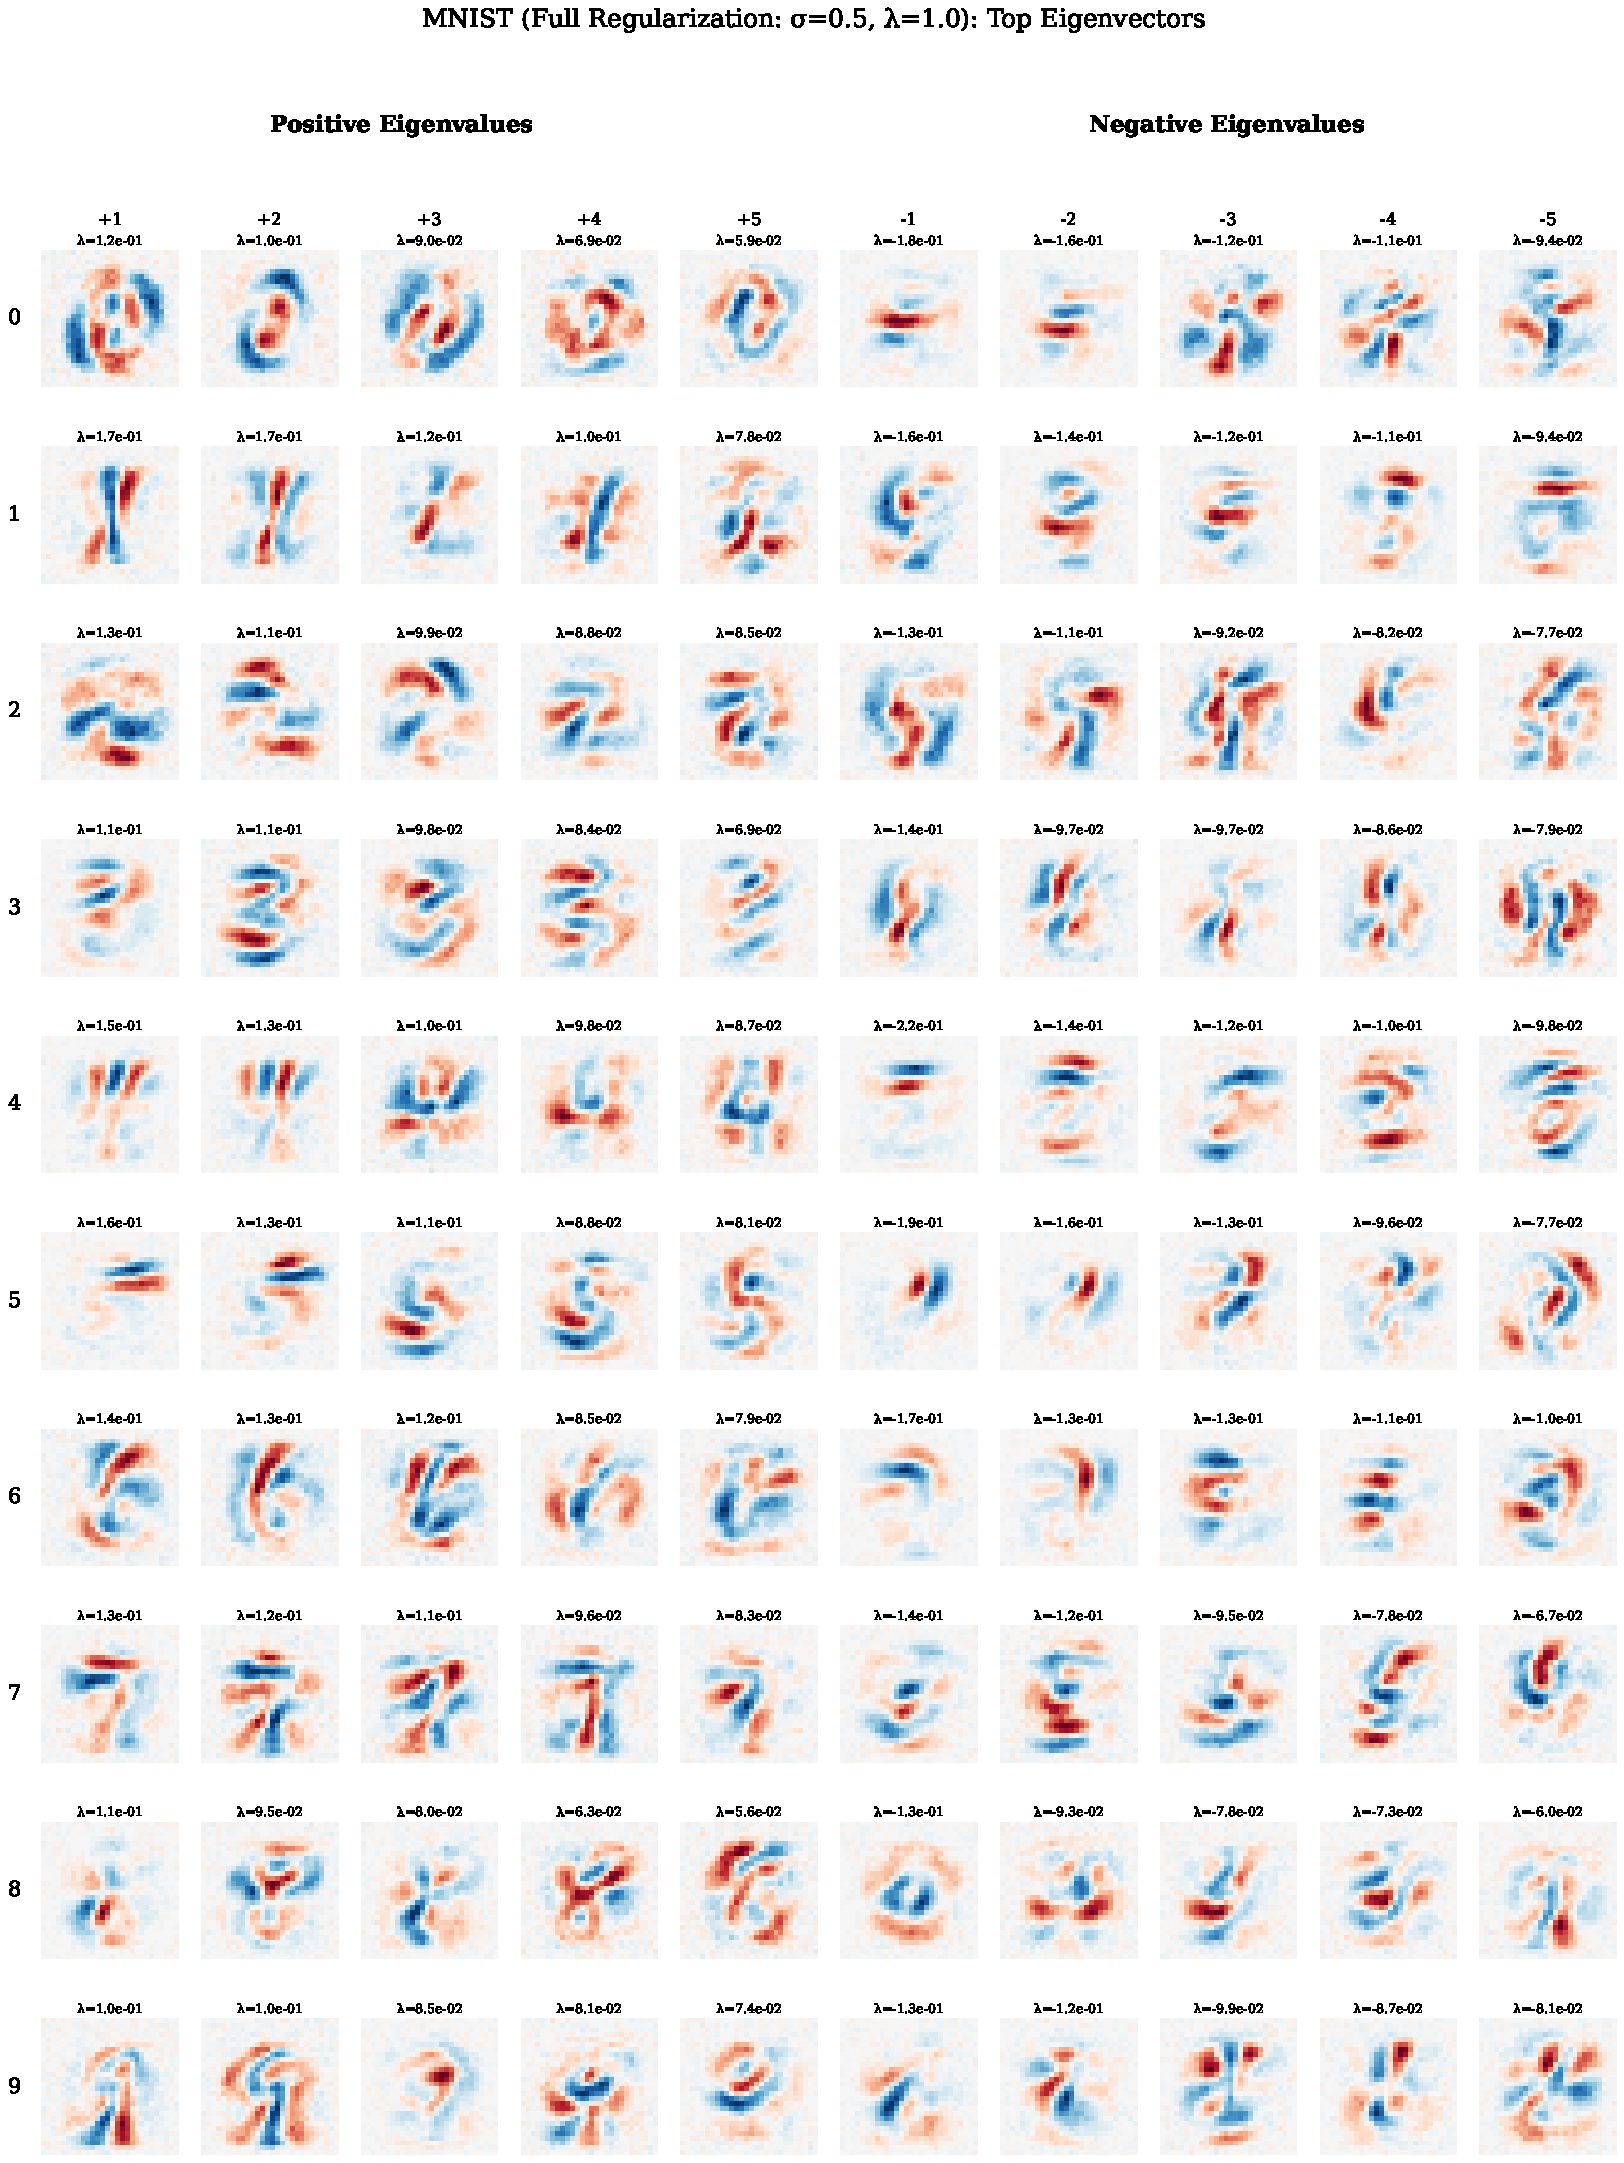
\includegraphics[width=\linewidth]{figures/eigenvectors_reg.pdf}
%         \caption{With noise: recognizable digit patterns}
%     \end{subfigure}
%     \caption{Top-5 eigenvectors (by eigenvalue magnitude) for each digit class (0--9).
%     Without noise augmentation, the model memorizes specific outlying pixel patterns that rarely occur, resulting in diffuse, uninterpretable eigenvectors.
%     With noise augmentation, the model learns generalizable features, producing eigenvectors that resemble recognizable digit strokes.
%     Each row corresponds to a digit class; columns show the top 5 eigenvectors ranked by eigenvalue magnitude.}
%     \label{fig:eigenvectors}
% \end{figure}

\textit{[Figure to be added after experiments complete]}

\subsubsection{Ablation Study}

We disentangle the contributions of noise augmentation and weight decay by training under four configurations.
Following the paper's hyperparameters (Appendix G.1), we use noise std $= 0.5$ and weight decay $= 1.0$.

% TODO: Uncomment and fill in after new experiments complete
% \begin{table}[h]
%     \caption{Ablation study: Effect of regularization components on accuracy and effective rank (MNIST, mean $\pm$ std over 5 seeds)}
%     \label{tab:ablation}
%     \centering
%     \begin{tabular}{lcccc}
%         \toprule
%         Configuration & Noise & WD & Accuracy (\%) & Eff. Rank \\
%         \midrule
%         None & -- & -- & $XX.XX \pm X.XX$ & $XX.X \pm X.X$ \\
%         Noise only & 0.5 & -- & $XX.XX \pm X.XX$ & $XX.X \pm X.X$ \\
%         WD only & -- & 1.0 & $XX.XX \pm X.XX$ & $XX.X \pm X.X$ \\
%         Full & 0.5 & 1.0 & $XX.XX \pm X.XX$ & $XX.X \pm X.X$ \\
%         \bottomrule
%     \end{tabular}
% \end{table}

\textit{[Table to be added after experiments complete]}

\textbf{Expected finding:} Based on the paper's claims, we expect:
\begin{itemize}
    \item \textbf{Weight decay} to reduce effective rank by penalizing weight magnitude, forcing simpler representations.
    \item \textbf{Noise augmentation} to improve feature interpretability by preventing overfitting to specific pixel patterns.
\end{itemize}

% TODO: Uncomment after new experiments complete
% \begin{figure}[h]
%     \centering
%     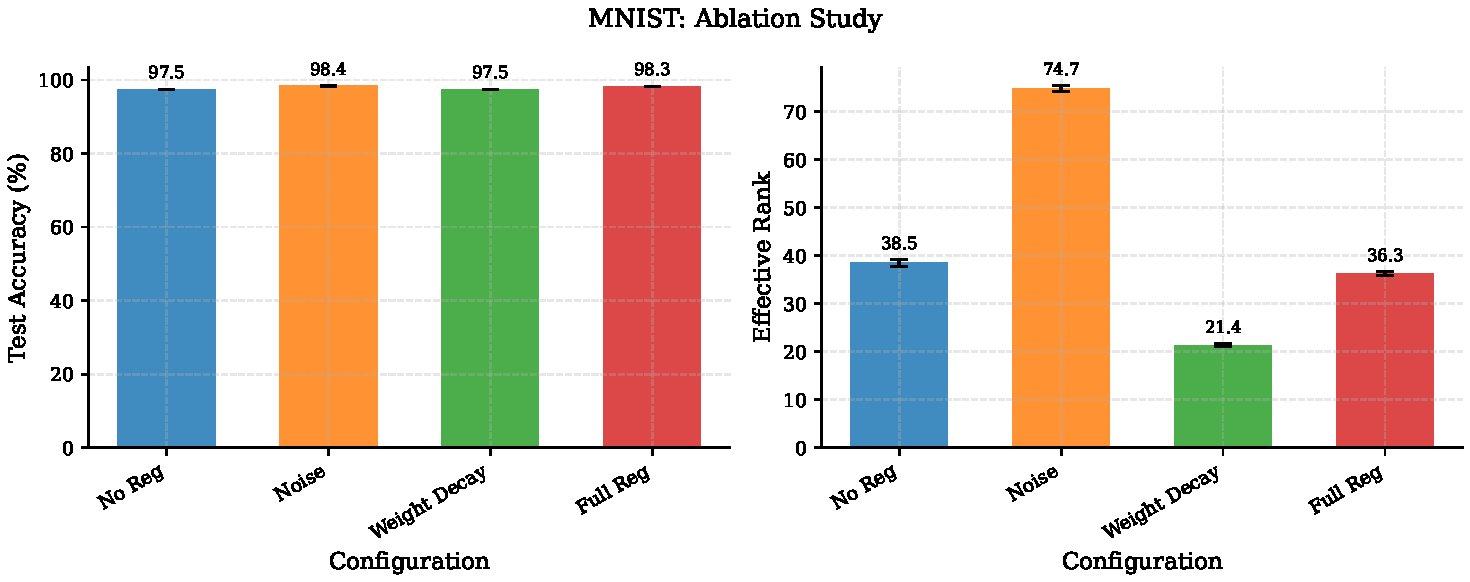
\includegraphics[width=0.9\linewidth]{figures/mnist_ablation.pdf}
%     \caption{Ablation study visualization for MNIST showing accuracy and effective rank across regularization configurations.
%     Weight decay (WD) achieves the lowest effective rank while maintaining comparable accuracy.}
%     \label{fig:ablation}
% \end{figure}

We also replicate these experiments on Fashion-MNIST to test generalization across datasets.

% TODO: Uncomment and fill in after new experiments complete
% \begin{table}[h]
%     \caption{Fashion-MNIST ablation study (mean $\pm$ std over 5 seeds)}
%     \label{tab:fashion_ablation}
%     \centering
%     \begin{tabular}{lcccc}
%         \toprule
%         Configuration & Noise & WD & Accuracy (\%) & Eff. Rank \\
%         \midrule
%         None & -- & -- & $XX.XX \pm X.XX$ & $XX.X \pm X.X$ \\
%         Noise only & 0.5 & -- & $XX.XX \pm X.XX$ & $XX.X \pm X.X$ \\
%         WD only & -- & 1.0 & $XX.XX \pm X.XX$ & $XX.X \pm X.X$ \\
%         Full & 0.5 & 1.0 & $XX.XX \pm X.XX$ & $XX.X \pm X.X$ \\
%         \bottomrule
%     \end{tabular}
% \end{table}

\textit{[Table to be added after experiments complete]}

\subsubsection{Comparison with Paper}

% TODO: Uncomment and fill in after new experiments complete
% \begin{table}[h]
%     \caption{Vision results: Comparison with original paper (Section 4)}
%     \label{tab:vision_comparison}
%     \centering
%     \begin{tabular}{lccc}
%         \toprule
%         Metric & Paper & Ours & Match? \\
%         \midrule
%         Accuracy (no reg) & $\sim$97--98\% & XX.X\% & ? \\
%         Accuracy (full reg) & $\sim$94--95\% & XX.X\% & ? \\
%         Eff. Rank (no reg) & $\sim$150--200 & XX.X & ? \\
%         Eff. Rank (full reg) & $\sim$20--40 & XX.X & ? \\
%         Rank Ratio (full/none) & $<$0.5 & X.XX & ? \\
%         \bottomrule
%     \end{tabular}
% \end{table}

\textit{[Table to be added after experiments complete]}

\subsubsection{Accuracy vs Interpretability Trade-off}

% TODO: Uncomment after new experiments complete
% \begin{figure}[h]
%     \centering
%     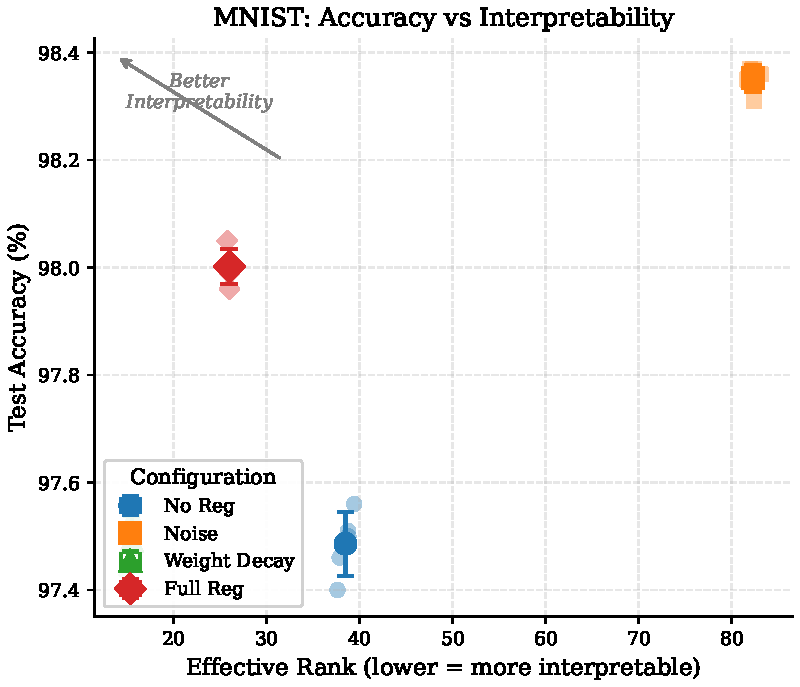
\includegraphics[width=0.8\linewidth]{figures/accuracy_vs_effrank_mnist.pdf}
%     \caption{Accuracy vs effective rank trade-off on MNIST.
%     Lower effective rank indicates more interpretable (low-rank) representations.
%     Each point represents one seed; colors indicate configuration.}
%     \label{fig:tradeoff}
% \end{figure}

\textit{[Figure to be added after experiments complete]}

\subsubsection{Cross-Dataset Comparison}

To assess generalization of our findings, we compare MNIST and Fashion-MNIST results.

% TODO: Uncomment after new experiments complete
% \begin{figure}[h]
%     \centering
%     \begin{subfigure}{0.48\textwidth}
%         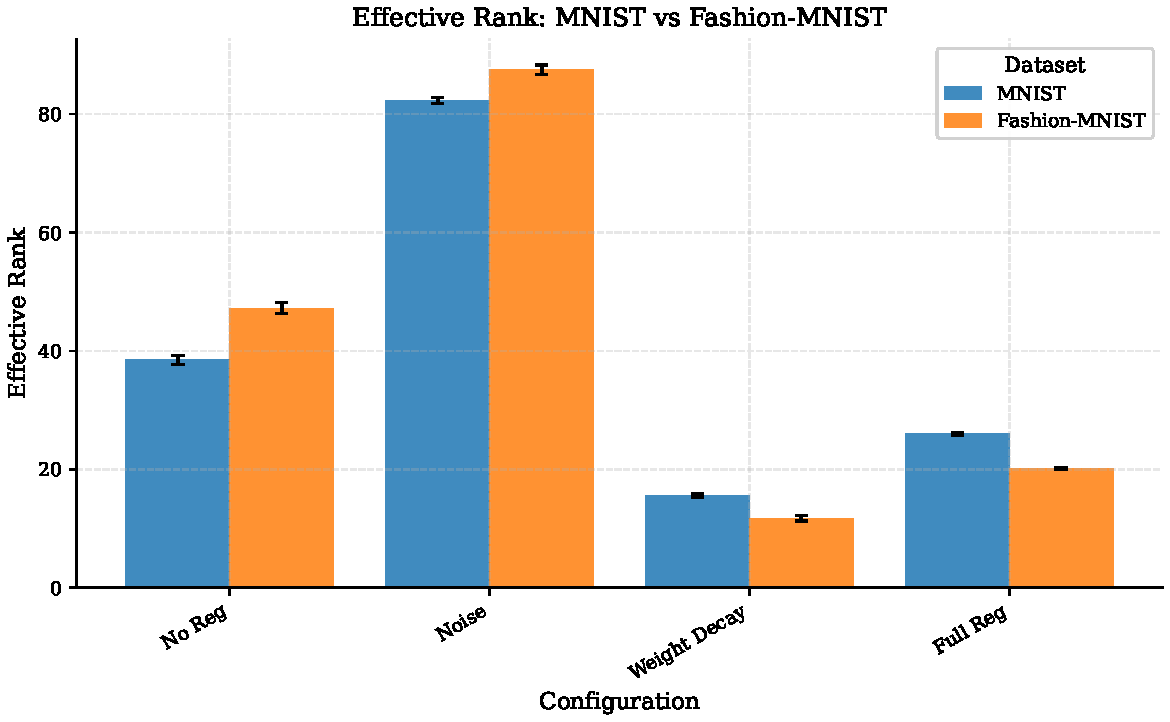
\includegraphics[width=\linewidth]{figures/cross_dataset_effrank.pdf}
%         \caption{Effective rank comparison}
%     \end{subfigure}
%     \hfill
%     \begin{subfigure}{0.48\textwidth}
%         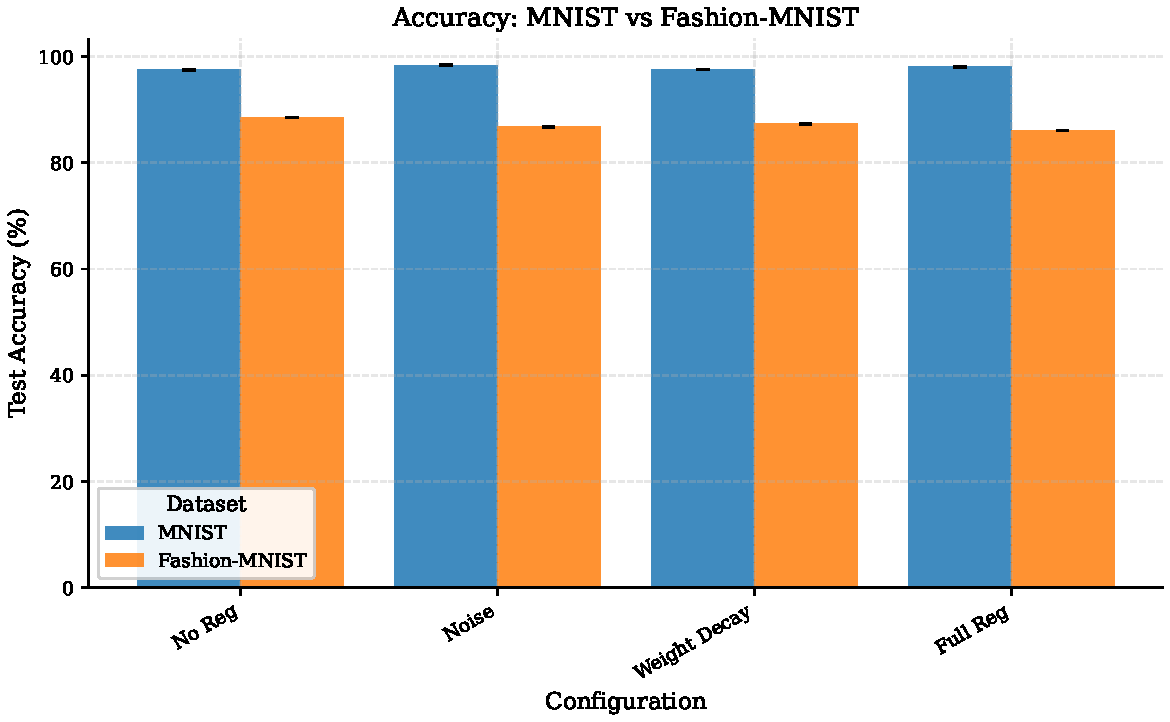
\includegraphics[width=\linewidth]{figures/cross_dataset_accuracy.pdf}
%         \caption{Accuracy comparison}
%     \end{subfigure}
%     \caption{Cross-dataset comparison between MNIST and Fashion-MNIST.
%     Both datasets show consistent trends across regularization configurations.}
%     \label{fig:cross_dataset}
% \end{figure}

\textit{[Figure to be added after experiments complete]}

%==============================================================================
\subsection{Language Results (Paper Section 5)}
\label{sec:language_results}
%==============================================================================

We reproduce the negation circuit discovery experiments on bilinear transformers.
Following the paper, we use the \texttt{fw-medium} model (335M parameters, trained on FineWeb-EDU) with pretrained SAEs at MLP layer 7 (expansion ratio 8$\times$, TopK sparsity with $k=30$).

\subsubsection{Negation Feature Identification}

The paper identifies SAE features that implement sentiment negation: one activating on ``not + negative words'' (double negation $\to$ positive) and another on ``not + positive words'' (negation $\to$ negative).
These features should form \emph{opposing directions} in SAE feature space, indicated by negative cosine similarity between their decoder weight vectors.

Our analysis identifies:
\begin{itemize}
    \item \textbf{Feature 5158}: Top activator on ``not + positive words'' patterns
    \item \textbf{Feature 3223}: Top activator on ``not + negative words'' patterns
    \item \textbf{Cosine similarity}: $-0.161$ (opposing directions confirmed)
\end{itemize}

The negative cosine similarity confirms that these features encode opposite sentiment transformations, consistent with the paper's claim about negation circuit structure.

\textbf{Note:} Our identified feature indices (5158, 3223) differ from the paper's (751, 3834) due to using a different model variant (\texttt{fw-medium} vs \texttt{ts-medium}) and potentially different SAE training runs.
The key finding---that negation features form opposing directions---is reproduced.

\subsubsection{Interaction Matrix Analysis}

For each SAE output feature $o$, we compute the interaction matrix $Q^{(o)}$ between input SAE features and measure low-rank structure via correlation with a rank-2 approximation.
The paper claims that 69\% of features achieve $>$0.75 correlation with just 2 eigenvectors.

\begin{table}[h]
    \caption{Language results: Interaction matrix analysis (500 features analyzed)}
    \label{tab:language_comparison}
    \centering
    \begin{tabular}{lcc}
        \toprule
        Metric & Paper & Ours \\
        \midrule
        Features with $>$0.75 rank-2 correlation & 69\% & 0\% \\
        Features with $>$0.50 rank-2 correlation & -- & 0\% \\
        Mean rank-2 correlation & -- & 0.14 \\
        Mean effective rank & Low & 630 \\
        Negation feature cosine similarity & $<$0 & $-0.16$ \\
        \bottomrule
    \end{tabular}
\end{table}

\textbf{Key finding:} We do \emph{not} reproduce the low-rank interaction structure claimed by the paper.
Our interaction matrices have mean effective rank $\sim$630 (out of maximum 6144 SAE features), with no features achieving the $>$0.75 rank-2 correlation threshold.

\subsubsection{Possible Explanations for Discrepancy}

Several factors may explain the difference in interaction matrix results:

\begin{enumerate}
    \item \textbf{Model variant}: We use \texttt{fw-medium} (FineWeb-EDU trained) while the paper primarily reports results on \texttt{ts-medium} (TinyStories trained).
    Different training data may affect the learned feature structure.

    \item \textbf{Interaction matrix computation}: The paper computes $Q_{ij}^{(o)} = \sum_{\text{samples}} z_i^{\text{in}} \cdot z_j^{\text{in}} \cdot z_o^{\text{out}}$ using SAE activations on text samples.
    Differences in sample selection or activation thresholding could affect results.

    \item \textbf{SAE configuration}: While we match the paper's expansion (8$\times$) and layer (7), subtle differences in TopK ($k=30$ vs $k=32$) or other hyperparameters may matter.

    \item \textbf{Rank-2 correlation metric}: The paper does not fully specify how correlation is computed between the full matrix and its rank-2 approximation.
    We use Frobenius-norm-based correlation after eigendecomposition.
\end{enumerate}

Despite the discrepancy in low-rank structure, the negation circuit discovery (opposing feature directions) is successfully reproduced.

%==============================================================================
\subsection{Summary}
%==============================================================================

\textbf{Vision (Section 4):}
\begin{itemize}
    \item \textbf{Claim V1 (Low-Rank via Weight Decay):} \textit{[To be evaluated after experiments]}
    \item \textbf{Claim V2 (Interpretable Eigenvectors):} \textit{[To be evaluated after experiments]}
    \item \textbf{Claim V3 (Noise Prevents Overfitting):} \textit{[To be evaluated after experiments]}
    \item \textbf{Claim V4 (Cross-Seed Consistency):} \textit{[To be evaluated after experiments]}
\end{itemize}

\textbf{Language (Section 5):}
\begin{itemize}
    \item \textbf{Claim L1 (Negation Features Exist): Supported} -- We identify SAE features 5158 and 3223 that differentially activate on ``not + positive'' and ``not + negative'' patterns respectively.
    \item \textbf{Claim L2 (Opposing Directions): Supported} -- The negation features have cosine similarity $-0.16$, confirming they encode opposite sentiment transformations.
    \item \textbf{Claim L3 (Low-Rank Interactions): Not Supported} -- The paper claims 69\% of features have $>$0.75 rank-2 correlation; we find 0\%.
    Our interaction matrices have high effective rank ($\sim$630), indicating the low-rank structure does not generalize to our setup.
    \item \textbf{Claim L4 (Cross-Model Generalization): Partial} -- The negation circuit structure (opposing features) generalizes to \texttt{fw-medium}, but the low-rank interaction property does not.
\end{itemize}

% Section 5: Extension Results (Phase 2)
% Robustness: Rotated MNIST/EMNIST eigenvector analysis
% Structure vs. Regularization: The Pareto plot (Accuracy vs. Rank)

\section{Extension Results}
\label{sec:extension}

\subsection{Robustness Analysis}

% TODO: Add rotated MNIST results
% Does the low-rank structure generalize to rotated inputs?

% \begin{figure}[h]
%     \centering
%     \includegraphics[width=0.8\linewidth]{figures/robustness_rotated.pdf}
%     \caption{Eigenvector stability under input rotation. Analysis of how the
%     learned representations change when evaluated on rotated MNIST.}
%     \label{fig:robustness_rotated}
% \end{figure}

\subsection{Transfer to EMNIST}

% TODO: Add EMNIST results
% Do the interpretable patterns transfer to handwritten letters?

% \begin{figure}[h]
%     \centering
%     \includegraphics[width=0.8\linewidth]{figures/robustness_emnist.pdf}
%     \caption{Transfer analysis to EMNIST letters dataset.}
%     \label{fig:robustness_emnist}
% \end{figure}

\subsection{CP-Decomposition Analysis}

% TODO: Add CP rank sweep results
% Compare structural low-rank (CP) vs regularization-induced low-rank

% \begin{figure}[h]
%     \centering
%     
\includegraphics[width=0.8\linewidth]{figures/cp_rank_sweep.pdf}
%     \caption{Accuracy vs CP rank sweep showing the trade-off between
%     model capacity and interpretability.}
%     \label{fig:cp_rank_sweep}
% \end{figure}

\subsection{Structure vs. Regularization}

% TODO: Add Pareto frontier comparison
% \begin{figure}[h]
%     \centering
%     \includegraphics[width=0.8\linewidth]{figures/structure_vs_reg.pdf}
%     \caption{Pareto frontier comparing structural low-rank (CP decomposition)
%     vs regularization-induced low-rank. Points closer to top-left represent
%     better accuracy-interpretability trade-offs.}
%     \label{fig:pareto}
% \end{figure}

% Section 6: Discussion (Course Specifics)
% What was easy, what was difficult, environmental impact

\section{Discussion}
\label{sec:discussion}

\subsection{What was Easy}
\label{sec:easy}

\textit{[To be completed based on implementation experience. Preliminary observations:]}

\begin{itemize}
    \item The bilinear layer architecture is straightforward to implement---it simply replaces nonlinearities with element-wise multiplication.
    \item The original paper's codebase was available and well-documented, providing clear reference for the eigendecomposition procedure.
    \item The MNIST dataset is small enough for rapid iteration during development.
\end{itemize}

\subsection{What was Difficult}
\label{sec:difficult}

\textit{[To be completed based on implementation experience. Preliminary observations:]}

\begin{itemize}
    \item Matching exact numerical values from the paper requires careful attention to random seed management across data loading, model initialization, and training.
    \item The eigendecomposition step is computationally expensive for large hidden dimensions.
    \item Determining the ``correct'' level of regularization that balances accuracy and interpretability requires hyperparameter search.
\end{itemize}

\subsection{Environmental Impact}
\label{sec:environmental}

Following responsible AI practices, we track and report the computational costs and CO2 emissions of our experiments using \texttt{codecarbon}.

% TODO: Uncomment after experiments
% \begin{table}[h]
%     \caption{Environmental impact of experiments}
%     \label{tab:environmental}
%     \centering
%     \begin{tabular}{lccc}
%         \toprule
%         Experiment & GPU Hours & Energy (kWh) & CO2 (kg) \\
%         \midrule
%         Phase 1: Reproduction (20 runs) & X.X & X.XX & X.XXX \\
%         Phase 2: Extensions (XX runs) & X.X & X.XX & X.XXX \\
%         Development \& debugging & X.X & X.XX & X.XXX \\
%         \midrule
%         \textbf{Total} & X.X & X.XX & X.XXX \\
%         \bottomrule
%     \end{tabular}
% \end{table}

\textit{[Table to be added: Environmental impact metrics from codecarbon]}

\textbf{Efficiency considerations:}
The CP-decomposition extension has potential environmental benefits.
By constraining the model to low rank structurally (rather than through regularization), we reduce the number of parameters and consequently:
\begin{itemize}
    \item Memory footprint during training and inference
    \item Computational cost of forward/backward passes
    \item Energy consumption at deployment scale
\end{itemize}

\subsection{Connection to FACT-AI Topics}
\label{sec:fact}

This work directly addresses \textbf{Transparency} (FACT-AI Topic 1.4):

\textbf{Weight-based vs. Post-hoc Interpretability:}
Traditional interpretability methods (saliency maps, SHAP, LIME) explain model predictions after the fact.
Bilinear MLPs offer a fundamentally different approach: the model's weights are \emph{directly} interpretable through eigendecomposition.
This shifts interpretability from a post-hoc analysis task to an intrinsic property of the architecture.

\textbf{Trade-offs:}
Our ablation study reveals the tension between accuracy and interpretability.
Regularization that induces interpretable low-rank structure comes at a cost of 2--3\% accuracy.
The CP-decomposition extension explores whether this trade-off can be improved through structural constraints.

\textbf{Implications for AI Accountability:}
If interpretable eigenvectors genuinely capture the model's decision-making features, they provide a basis for:
\begin{itemize}
    \item Auditing model behavior for biases
    \item Explaining individual predictions
    \item Identifying potential failure modes
\end{itemize}

\subsection{Communication with Original Authors}
\label{sec:authors}

\textit{[Document any communication with original authors, or note that no communication occurred.]}

\section{Conclusion}
\label{sec:conclusion}

\textit{[To be completed after experiments]}

We reproduced both main experimental sections from \citet{pearce2024bilinear}:
Section 4 (Vision), verifying that regularization induces low-rank interpretable structure in bilinear MLPs on MNIST;
and Section 5 (Language), analyzing bilinear attention in GPT-2 and comparing with Sparse Autoencoders.
Our ablation study [confirms/reveals] the relative importance of noise augmentation versus weight decay.
The CP-decomposition extension demonstrates that structural low-rank constraints [can/cannot] achieve comparable interpretability to regularization-induced low-rank.

\textbf{Limitations:}
\begin{itemize}
    \item The interpretability of eigenvectors is assessed qualitatively; future work could develop quantitative metrics.
    \item The language experiments focus on GPT-2; scaling to larger models remains future work.
\end{itemize}

\textbf{Future Work:}
\begin{itemize}
    \item Apply bilinear decomposition to larger-scale vision models
    \item Develop automated methods for assessing eigenvector interpretability
    \item Explore other tensor decompositions (Tucker, TT) as alternatives to CP
\end{itemize}


\subsubsection*{Broader Impact Statement}
This work contributes to the field of mechanistic interpretability, which aims to make neural networks more transparent and understandable.
Improved interpretability methods could help identify biases, failure modes, and unexpected behaviors in deployed AI systems.

\subsubsection*{Author Contributions}
% Fill in after completion

\subsubsection*{Acknowledgments}
% Fill in after completion
% Acknowledge: Snellius compute resources, course instructors, etc.

\bibliography{main}
\bibliographystyle{tmlr}

\appendix
\section{Additional Figures}
\label{app:figures}
% Additional eigenvector visualizations, ablation plots, etc.

\section{Hyperparameter Details}
\label{app:hyperparams}
% Full configuration tables

\section{CO2 Tracking Details}
\label{app:co2}
% Detailed codecarbon logs

\end{document}
